\documentclass[tikz,border=4pt]{standalone}

\usepackage{amsmath}
\usepackage{amssymb}
\usepackage{xcolor}
\usepackage{tikz}


\usetikzlibrary{
    arrows,
    arrows.meta,
    automata,
    backgrounds,
    calc,
    decorations.pathreplacing,
    fit,
    matrix,
    positioning,
    shapes,
    shapes.arrows,
    shapes.geometric,
    shapes.multipart
}



\tikzset{
  start/.style={
    rectangle,
    rounded corners,
    minimum width=3.5cm,
    minimum height=1cm,
    text centered,
    text width=3cm,
    draw=black,
    fill=green!20
  },
  stop/.style={
    rectangle,
    rounded corners,
    minimum width=3cm,
    minimum height=1cm,
    text centered,
    text width=2.5cm,
    draw=black,
    fill=red!20
  },
  decision/.style={
    diamond,
    aspect=2,
    minimum width=3cm,
    minimum height=1.2cm,
    text centered,
    text width=2.5cm,
    inner sep=1pt,
    draw=black,
    fill=yellow!20
  },
  process/.style={
    rectangle,
    minimum width=3cm,
    minimum height=1cm,
    text centered,
    text width=2.7cm,
    draw=black,
    fill=blue!10
  },
  arrow/.style={
    thick,
    -{Stealth}
  }
}


\usetikzlibrary{
  arrows.meta,
  positioning,
  shapes.geometric
}

\tikzset{
  start/.style={
    rectangle,
    rounded corners,
    minimum width=3.5cm,
    minimum height=1cm,
    text centered,
    text width=3cm,
    draw=black,
    fill=green!20
  },
  stop/.style={
    rectangle,
    rounded corners,
    minimum width=3cm,
    minimum height=1cm,
    text centered,
    text width=2.5cm,
    draw=black,
    fill=red!20
  },
  decision/.style={
    diamond,
    aspect=2,
    minimum width=3cm,
    minimum height=1.2cm,
    text centered,
    text width=2.5cm,
    inner sep=1pt,
    draw=black,
    fill=yellow!20
  },
  io/.style={
    trapezium,
    trapezium left angle=70,
    trapezium right angle=110,
    minimum width=3.5cm,
    minimum height=1cm,
    text centered,
    text width=3cm,
    draw=black,
    fill=blue!20
  },
  arrow/.style={
    thick,
    -{Stealth}
  }
}

\input{../jpk.inc}


\begin{document}

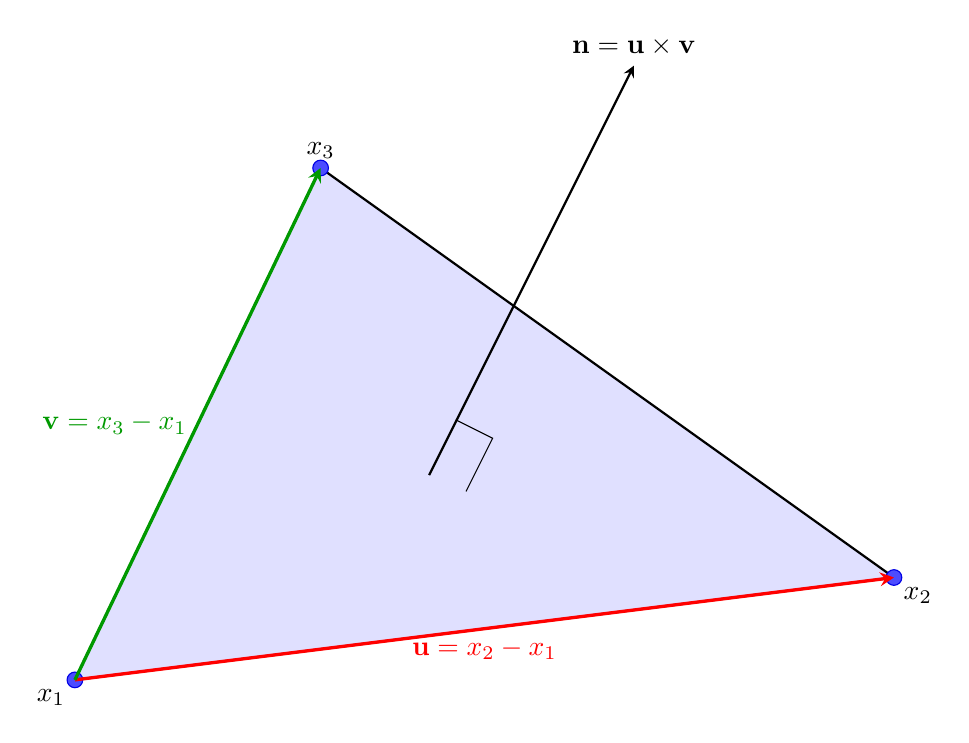
\begin{tikzpicture}[ scale=2.6, vertex/.style={ circle, fill=blue!70, draw=blue!90!black, inner sep=2pt }, vector/.style={ ->, >=stealth, very thick } ] 
\coordinate (P1) at (0,0); 
  \coordinate (P2) at (4,0.5); 
  \coordinate (P3) at (1.2,2.5); 
\fill[blue!12] (P1)--(P2)--(P3)--cycle; 
  \draw[thick] (P1)--(P2)--(P3)--cycle; 
\node[vertex] at (P1) {}; 
  \node[below left] at (P1) {$\V{x}_1$}; 
  \node[vertex] at (P2) {}; 
  \node[below right] at (P2) {$\V{x}_2$}; 
  \node[vertex] at (P3) {}; 
  \node[above] at (P3) {$\V{x}_3$}; 
\draw[vector, red] (P1) -- (P2) node[midway, below] {$\mathbf{u}=\V{x}_2-\V{x}_1$}; \draw[vector, green!60!black] (P1) -- (P3) node[midway, left] {$\mathbf{v}=\V{x}_3-\V{x}_1$}; 
\coordinate (C) at (1.73,1.0); 
\draw[vector, thick] (C) -- ++(1.0,2.0) node[above] {$\mathbf{n}=\mathbf{u}\times\mathbf{v}$}; 
\draw[thin] ($(C)+(0.13,0.27)$) -- ++(0.18,-0.09) -- ++(-0.13,-0.26); 
\end{tikzpicture}

\end{document}
